% This must be in the first 5 lines to tell arXiv to use pdfLaTeX, which is strongly recommended.
\pdfoutput=1
% In particular, the hyperref package requires pdfLaTeX in order to break URLs across lines.

\documentclass[11pt, round]{article}

% Remove the "review" option to generate the final version.
\usepackage{acl}
\usepackage{gb4e}
\noautomath
% Standard package includes
\usepackage{times}
\usepackage{latexsym}

\usepackage{graphicx}
\usepackage{caption}
\usepackage{subcaption}
\graphicspath{{./img/}}

% For proper rendering and hyphenation of words containing Latin characters (including in bib files)
\usepackage[T1]{fontenc}
% For Vietnamese characters
% \usepackage[T5]{fontenc}
% See https://www.latex-project.org/help/documentation/encguide.pdf for other character sets

% This assumes your files are encoded as UTF8
\usepackage[utf8]{inputenc}

% This is not strictly necessary, and may be commented out,
% but it will improve the layout of the manuscript,
% and will typically save some space.
\usepackage{microtype}

\usepackage{natbib}
\bibliographystyle{plainnat}

\title{Do LSTMs Understand the Licensing of Negative Polarity Items?}

\author{Theo Sandstrom \\
  \texttt{theo.sandstrom@yale.edu} \\
  Trey Skidmore \\
  \texttt{trey.skidmore@yale.edu} \\
  Prastik Mohanraj \\
  \texttt{prastik.mohanraj@yale.edu}}

\begin{document}
\maketitle

\begin{abstract}
While LSTMs have proven themselves as powerful tools for language modeling tasks, the extent to which their generalizations are based on underlying syntactic structure remains an open area of inquiry. We focus our investigation on the relationship between negative polarity items (NPIs) and their licensors in English. We probe the model's representation of this relationship by computing the network's surprisal upon encountering NPIs in licensed and unlicensed environments. While we do observe that the inclusion of a licensor causes a significant reduction in model surprisal, we do not observe any change in surprisal depending on whether or not the licensor c-commands the negative polarity item. 
\end{abstract}

\section{Introduction}

The development of Recurrent Neural Networks (RNN) has been a recent hallmark of advancements in Natural Language Processing (NLP). The inherent ability for RNNs to learn and internalize a number of linguistic capabilities is evidenced by a large corpus of research in the utilization of RNNs for NLP tasks such as machine translation, language modeling, and syntactic parsing \cite{wilcox-etal-2018-rnn,gulordava2018colorless,jozefowicz2016exploring}. 

However, it is still largely unknown how such networks represent linguistic information internally. Historically, the majority of research on these networks has focused simply on evaluating and optimizing performance on applied NLP tasks. However, there has been a recent increase in literature probing inside of these black box models and evaluating the extent to which their success is based on surface level heuristics rather than genuinely extracting and interpreting structural properties of language, either syntactic or semantic \cite{lakretz2019emergence}.

One subset of RNNs, namely Long Short-Term Memory RNNs (LSTMs), has grown in utility in said extraction of structural properties of language. Wilcox et al. \shortcite{wilcox-etal-2018-rnn} researched the ability of LSTM models to learn the syntactic filler-gap dependency, the relationship between a filler word (in English, a wh- complementizer like \textit{what} or \textit{when}) and a gap word (in English, an empty syntactic position uniquely licensed by a filler word). Lakretz et al. \shortcite{lakretz2019emergence} similarly explored the ability of LSTM models to identify numerical agreement between verbs and their arguments. 

There is, though, little research investigating the feature of licensing of negative polarity items in language. Negative polarity items are a class of words that are only permitted to appear in certain ``negative'' contexts. For example, in English, negative polarity items include words like \textit{ever}, \textit{any}, and \textit{even}.
\begin{exe}
\ex \begin{xlist}
\ex \label{ex:example1} The boy did not ever give up.
\ex[*]{\label{ex:example2} The boy did ever give up.}
\ex[*]{\label{ex:example3} The boy who did not win did ever give up.}
\end{xlist}
\end{exe}
Considering Examples \ref{ex:example1} and \ref{ex:example2}, we note that the word \textit{ever} is only permitted to occur in a sentence when it is licensed by a word such as \textit{nobody} which provides a ``negative'' context. For this basic example, the relationhip between licensor and NPI would not be a particularly challenging task for a language model to learn; if it doesn't see any negative words in environment, then it won't predict an NPI. 

However, considering Example \ref{ex:example3}, we see that this simple heuristic fails. Despite the fact that the word \textit{not} preceeds the NPI, the sentence is still ungrammatical. This is because the relationship between the licensor and the negative polarity item is not based on linear word order but rather on the hierarchical structure of a sentence. In particular, for an NPI to be permissible, it must be c-commanded by a licensor. This c-command relation means that the NPI must be a sister of the licensor or a direct descendant of a sister node of the licensor \cite{ladusaw1980notion}.

Jumelet and Hupkes \shortcite{jumelet2018language} investigated neural language models for NPIs via analysis utilizing perplexity scores, defined as the exponent of the normalized negative log probability of different sentences, wherein the lower the perplexity score of a sentence is, the better a model was able to predict its tokens. Jumelet et al. \shortcite{jumelet2021language} similarly investigated neural language models for NPIs via analysis utilizing conditional probability distributions and a novel method ranking their model's decoder weights for all tokens based on their similarity with monotonicity weights in their sentence data sets. This is the general extent of the existing literature on NPIs, and neither study makes reference to the surprisal metric, which we introduce in Subsection \ref{sec:surpisal} and contend is a superior metric for analysis.

If a language model trained on a generic linguistic data set is able to predict the distribution of negative polarity items accurately, this would be evidence that the model is able to learn this feature of syntax, and in particular, that its internal representation captures hierarchical structure with enough fidelity to encapsulate the c-command relation.

\section{Methods}

\subsection{Language Model}

For our investigation, we trained a LSTM model on the WikiText-2 data set \cite{merity2016pointer}, which consists of over 2 million tokens from 600 Wikipedia articles, with a vocabulary size of 33,279. Our LSTM has an embedding layer, assigning 200-dimensional embeddings to each word in the vocabulary, and two recurrent layers, each with 650 hidden units. During training, we use dropout regularization as described in Srivastava et. al. \shortcite{srivastava2014dropout}, with a dropout rate set at 0.2. Optimization was performed using gradient descent, with a base learning rate of 0.2, which decreased exponentially whenever performance on the development set regressed.

The model can be found in the project's GitHub repository\footnote{\url{https://github.com/tsandstr/ling380-final-project}}.

\subsection{Surprisal}
\label{sec:surpisal}

We assess the ability of an LSTM to predict the distribution of negative polarity items by using the surprisal metric, as applied in Wilcox et. al. \shortcite{wilcox-etal-2018-rnn}. The metric is defined to be the log inverse probability:
\[ S(x_i) = -\log_2 P(x_i \, | \, h_{i-1}), \]
where $x_i$ is the current word, $h_{i-1}$ is the LSTM's hidden state before $x$ and the probability is given by the softmax activation. The surprisal is measured in bits because we take a base two logarithm.

A high surprisal metric means that, in the given context, a word was predicted with \textit{low} probability, and was therefore unexpected by the model. Intuitively, given a hidden state of the model at a current time step, the surprisal metric is a way to measure the whether the next word makes \textit{sense}. A direct correlation has been shown between language model surprisal metrics and  human sentence processing difficulty \cite{hale2001probabilistic,levy2008expectation,smith2013effect}. 

\section{Representation of Negative Polarity Items}

Negative polarity items have a variety of linguistic properties which we would like to probe. On the most basic level, they are only allowed to occur in negative contexts. More specifically, in order for an NPI to be licit, it must be c-commanded by its licensor. Another property is that NPIs are immune to intervening material separating the NPI from its licensor. In this section we  investigate whether LSTMs understand these three properties.

Our general approach to studying these properties of the dependency between NPI and licensor is as follows. We construct a number of test items containing negative polarity items, including variation in whichever independent variable we are curious about (e.g. whether or not the licensor c-commands the NPI). For each item, we construct two variants: one with a licensor, and one without a licensor. We define the licensing interaction to be the difference in surprisals between these two variants:
\[ \textrm{interaction} = S_{\textrm{no license}} - S_{\textrm{license}}. \]
A large licensing interaction suggests that, in a given test item, the presence of a licensor does dampen the model's surprisal at encountering an NPI, while a small licensing interactoin suggests that, in a given test item, the licensor does not dampen the surprisal.

In computing the licensing interaction, we measure surprisal in two different ways. First of all, we can measure the instantaneous surprisal of the model upon encountering an NPI. Secondly, we measure cumulative surprisal from the NPI to the end of its clause. We measure instantaneous surprisal because we expect the grammaticality of an NPI to have some local effect on the model's predictions. We measure cumulative surprisal because we expect the grammaticality of an NPI to have longer-reaching effects on the model's predictions for the whole sentence.

\subsection{Licensing of Negative Polarity Items}
\label{sec:basic}

As discussed in the introduction, negative polarity items are only grammatically allowable in negative contexts. The following examples demonstrate this fact because only the sentences with negative contexts (a,c) are grammatically permissible:
\begin{exe}
\ex\label{ex:license-1}
\begin{xlist}
\ex Bill is not here yet.
\ex[*]{Bill is here yet.}
\end{xlist}
\ex\label{ex:license-2}
\begin{xlist}
\ex They hired somebody without any talent.
\ex[*]{They hired somebody with any talent.}
\end{xlist}
\end{exe}
In this subsection, we confirm the hypothesis that surprisal metrics for NPIs are reduced in the presence of an appropriate licensor. As described above, we created 20 test items containing negative polarity items, and for each item, we constructed one variant with a licensor, and one without a licensor, as exemplified in Examples \ref{ex:license-1} and \ref{ex:license-2}.

Plotted in Figure \ref{fig:surprisal-basic-licensing} are graphs of surprisal on two generic examples; negative polarity items are assigned lower surprisal values by the model when they are found in grammatically licit environments. 

\begin{figure}
    \centering
    \subfloat[Grammatical]{{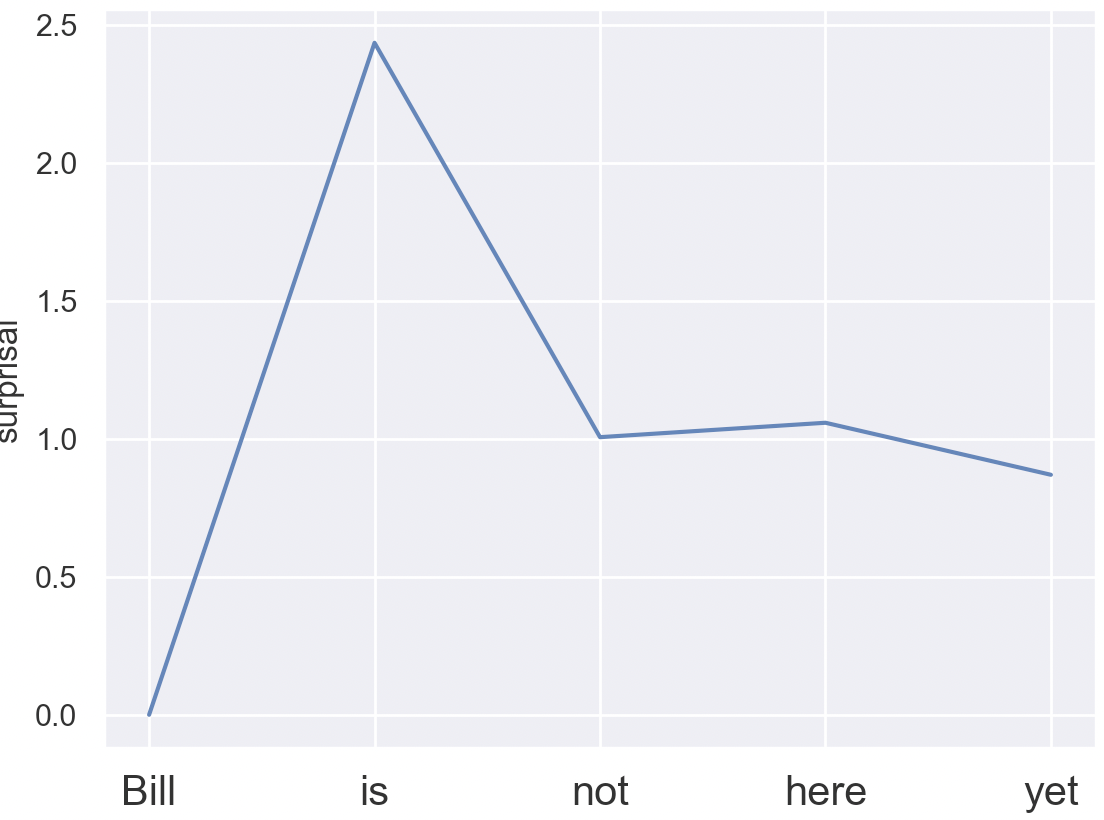
\includegraphics[width=.42\linewidth]{good1} }}
    \subfloat[Ungrammatical]{{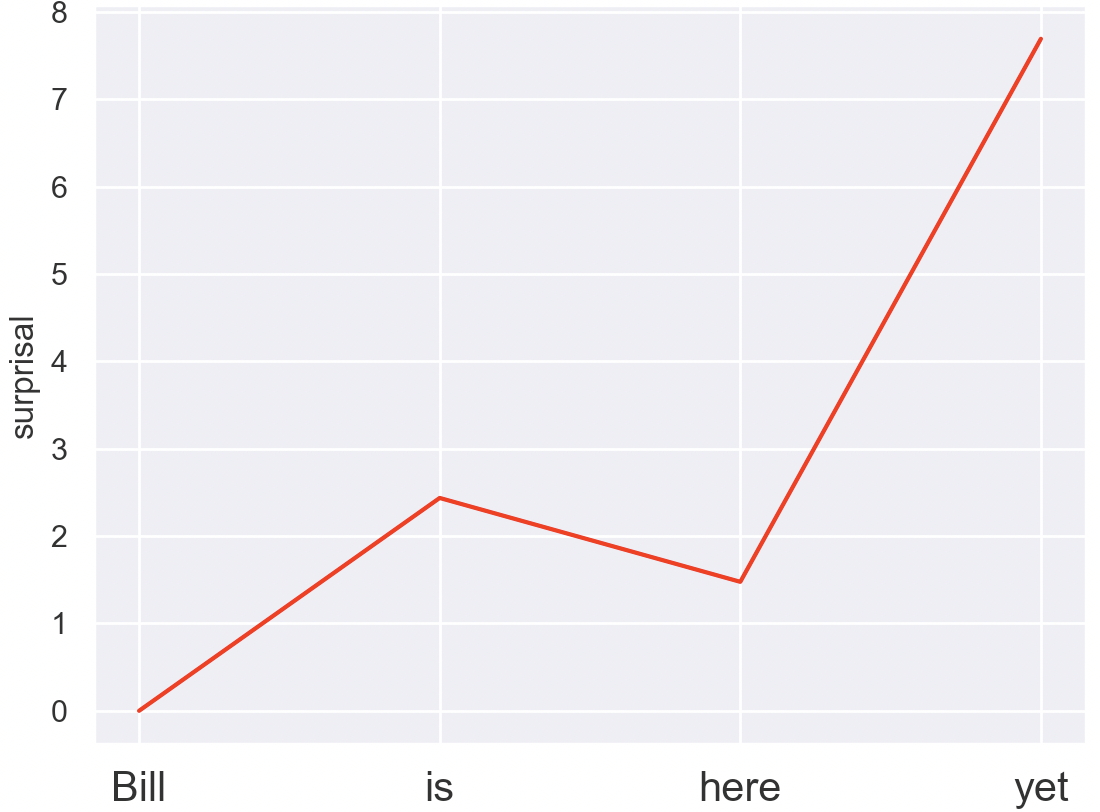
\includegraphics[width=.42\linewidth]{bad1} }}
    \qquad
    \subfloat[Grammatical]{{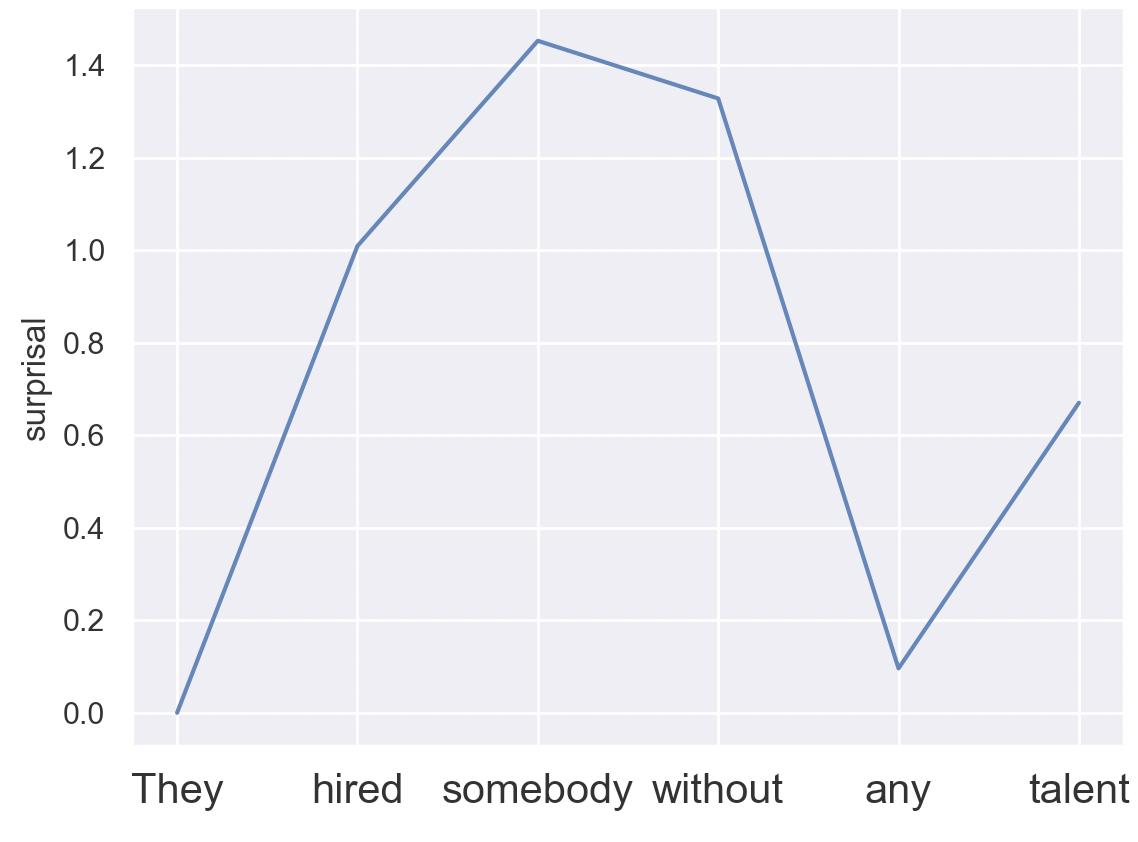
\includegraphics[width=.42\linewidth]{good2} }}
    \subfloat[Ungrammatical]{{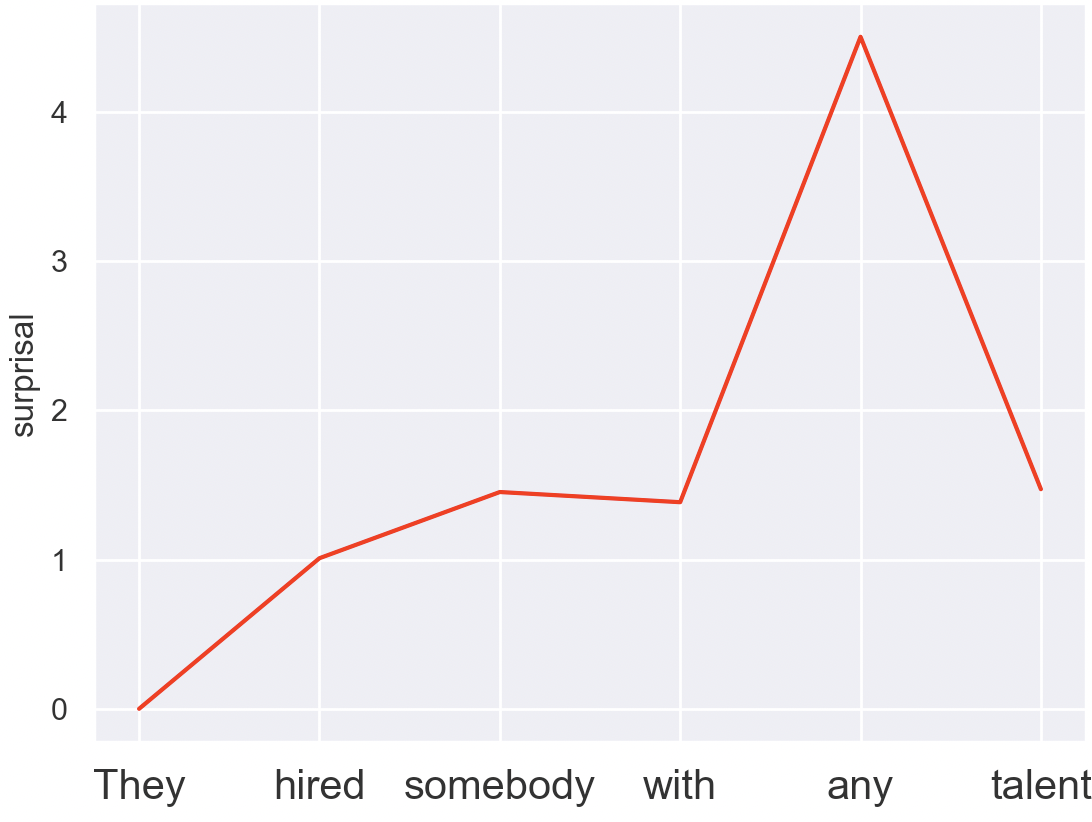
\includegraphics[width=.42\linewidth]{bad2} }}
    \caption{Plots of surprisal scores for words in the example sentences. Note that plots (a) and (c) are both contextually negative and plots (b) and (d) are positive. As expected, the surprisal score for the NPIs (\textit{yet} in plots (a) and (b) and \textit{any} in plots (c) and (d)) is much higher in positive contexts.}
    \label{fig:surprisal-basic-licensing}
\end{figure}

To determine the statistical significance of the surprisal scores of NPIs in different contexts, we computed surprisal scores for both variants of our 20 test items and computed the licensing interaction by taking pairwise differences. If the model had learned nothing at all about the NPI/licensor relation, we would expect the licensing interaction to be zero. However, if the model did learn to predict NPIs only in the presence of a licensor, then the licensing interaction should be positive. Our results are plotted in Figure \ref{fig:basic-detection-box-plot}.

\begin{figure}
    \centering
    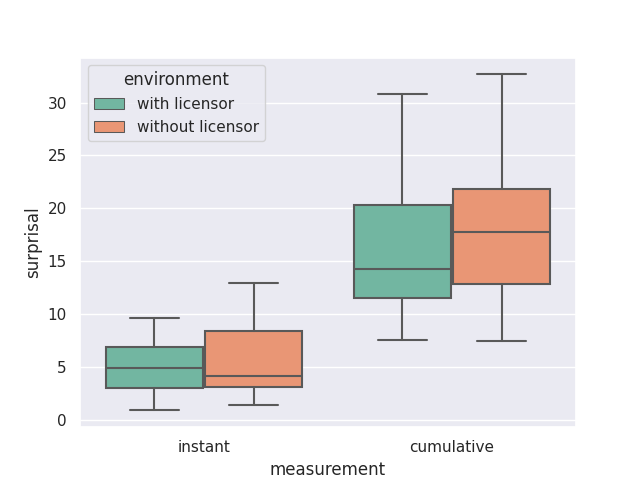
\includegraphics[width=0.5\textwidth]{surprisal-c-command-box-plot}
    \caption{Plots of surprisal scores in the presence of a licensor and without a licensor. As expected, surprisal tends to be higher in the environment with no licensor. Interstingly, \textit{median} instantaneous surprisal actually decreases when we include a licensor. However, this does not take into account the fact that our data set is paired; this is only captured when we apply a $t$-test to the licensing interaction.}
    \label{fig:basic-detection-box-plot}
\end{figure}

Measuring instantaneous surprisal upon encountering an NPI, we found a mean licensing interaction of 0.87, which we deemed significant ($t(19 = 1.82$, $p = 0.042$), so we reject the null hypothesis, concluding that the sentences containing a licensor had significantly lower suprisal than those without a licensor.

Measuring cumulative surprisal over the remainder of the clause, we found an even larger licensing interaction of 1.83, which we also deemed significant ($t(19) = 3.00$, $p = 0.004$).

Overall, this experiment shows that our LSTM model has at least a basic understanding of when negative polarity items should be expected.

\subsection{C-Command Relation Between Licensor and NPI}
\label{sec:c-command}

As discussed in the the Introduction, there are structural restrictions on the NPI licensing relationship. For an NPI construction to be grammatical, it is not sufficient that a negative licensor precede the NPI in terms of linear word order. In fact, the licensor must c-command the NPI in order for the construction to be grammatical.

Consider the sentences in Example \ref{ex:c-command}, each of which contains an embedded clause. In \ref{ex:c-command-nn} there is a negative licensor in both the embedded clause and the main clause, in \ref{ex:c-command-np} there is only a licensor in the embedded clause, in \ref{ex:c-command-pn} there is only a licensor in the main clause, and in \ref{ex:c-command-pp} there is no licensor at all.

\begin{exe}
\ex
\label{ex:c-command}
\begin{xlist}
\ex \label{ex:c-command-nn} That car which had no license plate was not even pulled over
\ex [*]{\label{ex:c-command-np} That car which had no license plate was even pulled over} 
\ex \label{ex:c-command-pn} That car which had a license plate was not even pulled over
\ex [*]{\label{ex:c-command-pp} That car which had a license plate was even pulled over}
\end{xlist}
\end{exe}

In this subsection we attempt to determine whether LSTMs are capable of understanding syntactic structure with regards to negative polarity items. In order to do this we designed 15 test items, each containing an embedded clause and an NPI. For each item, we generated four variants, as exemplified by those in Example \ref{ex:c-command}. If the model has learned that NPIs are only gramatical when they are c-commanded by a licensor, we should expect that the presence of a licensor in the main clause has a significant impact on surprisal, while the presence of a licensor in the embedded clause should not have a significant impact on surpisal. The results are visualized in Figure \ref{fig:c-command-box-plots}.

\begin{figure}
    \centering
    \begin{subfigure}[b]{0.5\textwidth}
        \centering
        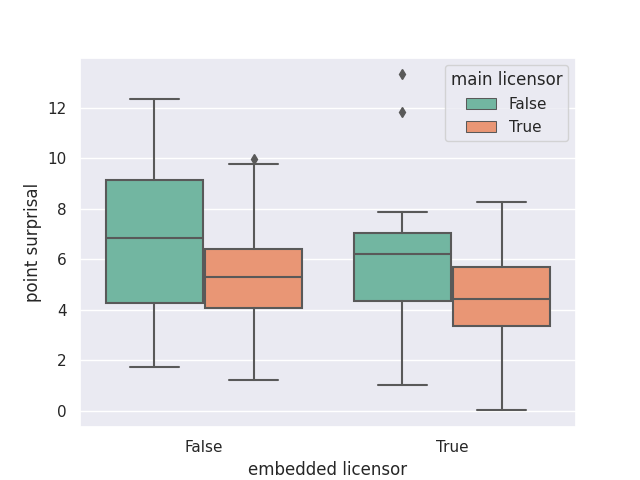
\includegraphics[width=\textwidth]{point_surprisal_c_command}
        \caption{Instantaneous surprisal}
    \end{subfigure}
    \hfill
    \begin{subfigure}[b]{0.5\textwidth}
        \centering
        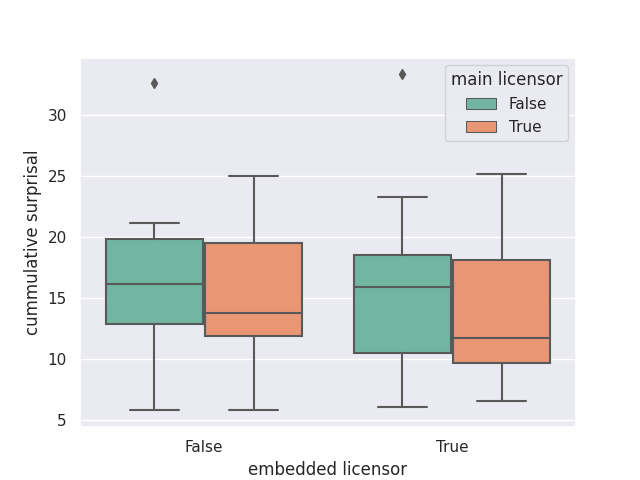
\includegraphics[width=\textwidth]{cummulative_surprisal_c_command}
        \caption{Cumulative surprisal}
    \end{subfigure}
    \caption{Surprisal values for sentences of the form in Example \ref{ex:c-command}. The environment of \ref{ex:c-command-nn} corresponds to the left most column, \ref{ex:c-command-np} corresponds to the third column, \ref{ex:c-command-pn} corresponds to the second column, and \ref{ex:c-command-pp} corresponds to the right most column.}
    \label{fig:c-command-box-plots}
\end{figure}


To test this hypothesis, we used two-way repeated measures ANOVA to analyze the effect of the embedded licensor and the main licensor on surprisal. The test showed a significant main effect of the main licensor on instantaneous surprisal ($F(1, 14) = 7.90$, $p = 0.014$). It also showed a significant main effect of the embedded licensor on instantaneous surprisal ($F(1, 14) = 8.22$, $p = 0.012$). It did not show any significant interaction between the main licensor and the embedded licensor ($F(1, 14) = 1.87$, $p = 0.193$).

Comparing the two statistically significant effects, we used partial-$\eta^2$ to measure the size of these effects (the (partial)-$\eta^2$ statistic for ANOVA is analogous to the $r^2$ statistic for linear regression, in that it described the proportion of variance in the dependent variable explained by each independent variable). We found that the effect size for the main licensor is $\eta_p^2 = 0.36$ and the effect size for the embedded licensor is $\eta_p^2 = 0.37$. Thus, both the main licensor and the embedded licensor have similar sized effets on instantaneous surprisal.

The fact that the interaction term is not significant means that the effect of the embedded licensor does not depend on the presence or lack of a main licensor. In other words, the effects of the licensors combine linearly.

These results tell us two things. First, they support the result of section \ref{sec:basic} that the presence of a licensor in the main clause reduces surprisal. Second, because there is a significant effect of the embedded licensor, we conclude that the model has not learned to generalize based on underlying sentence structure.

\subsection{Robustness to Intervening Material}
\label{sec:intervening}
Because the relation between licensor and NPI is based on the c-command relation rather than on linear word order, it is not sensitive to the amount of intervening material which occurs between the licensor and the NPI. In Example \ref{ex:intervening}, the NPI \textit{anymore} is licenced by the word \textit{not} in each sentence. The intervening prepositional phrases and relative clauses have no impact on the grammaticality of the sentences.
\begin{exe}
\ex \label{ex:intervening}
\begin{xlist}
\ex We do not go to the supermarket anymore.
\ex We do not go to the supermarket that is owned by Mark anymore.
\ex We do not go down the block to the supermarket that is owned by Mark anymore. 
\end{xlist}
\end{exe}
We showed in Section \ref{sec:basic} that LSTMs exhibit significantly higher surprisal when encountering an unlicensed NPI than a licensed NPI; however, the analysis in Section \ref{sec:c-command} suggests that the model is using a heuristic based on linear word order rather than taking into account the hierarchical structure of the sentence. Given this, we might predict that the amount of intervening material could have an impact on surprisal. 

To test the robustness of the model's predictions to intervening material, we first designed 21 test items containing NPIs. In constructing these items, we made sure to vary the amount of intervening material between the licensor and the NPI. Then, for each test item, we constructed two variations: one with a licensor and one without. For each item, we computed the licensing interaction, and then checked for a correlation between the amount of intervening material and the licensing interaction. Our results are visualized in Figure \ref{fig:intervening1}. We found no statistically signficant correlation between intervening length and either instantaneous licensing interaction ($p = 0.305$) or cumulative licensing interaction ($p = 0.485$). This suggests that the model's ability to predict NPI distribution is not affected by the mount of intervening material between the NPI and its licensor.

\begin{figure}
    \centering
    \begin{subfigure}[b]{0.45\textwidth}
        \centering
        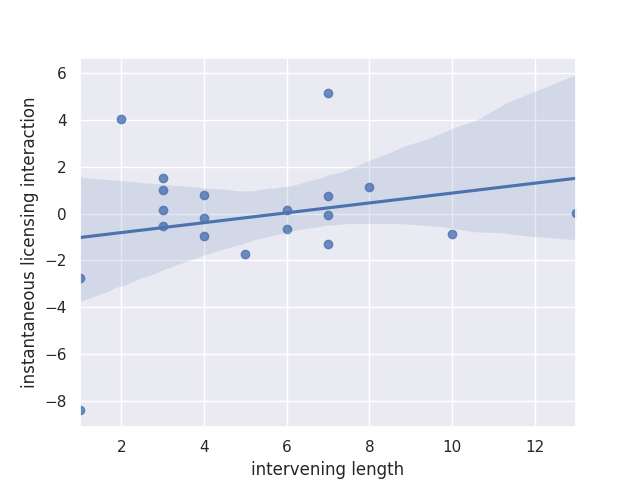
\includegraphics[width=\textwidth]{intervening_pnt_scatter}
        \caption{Instantaneous licensing interaction}
    \end{subfigure}
    \hfill
    \begin{subfigure}[b]{0.45\textwidth}
        \centering
        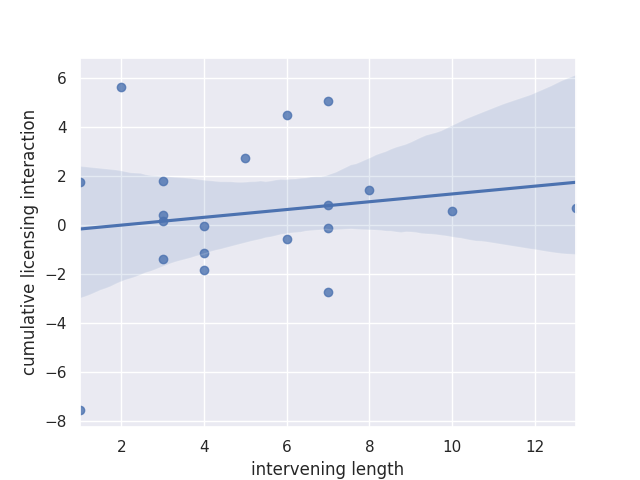
\includegraphics[width=\textwidth]{intervening_cum_scatter}
        \caption{Cumulative licensing interaction}
    \end{subfigure}
    \caption{Plots of licensing interaction of sentences given the amount of words in between the negative licensor and the NPI}
    \label{fig:intervening1}
\end{figure}
\begin{figure*}
    \centering
    \subfloat[Base Sentence]{{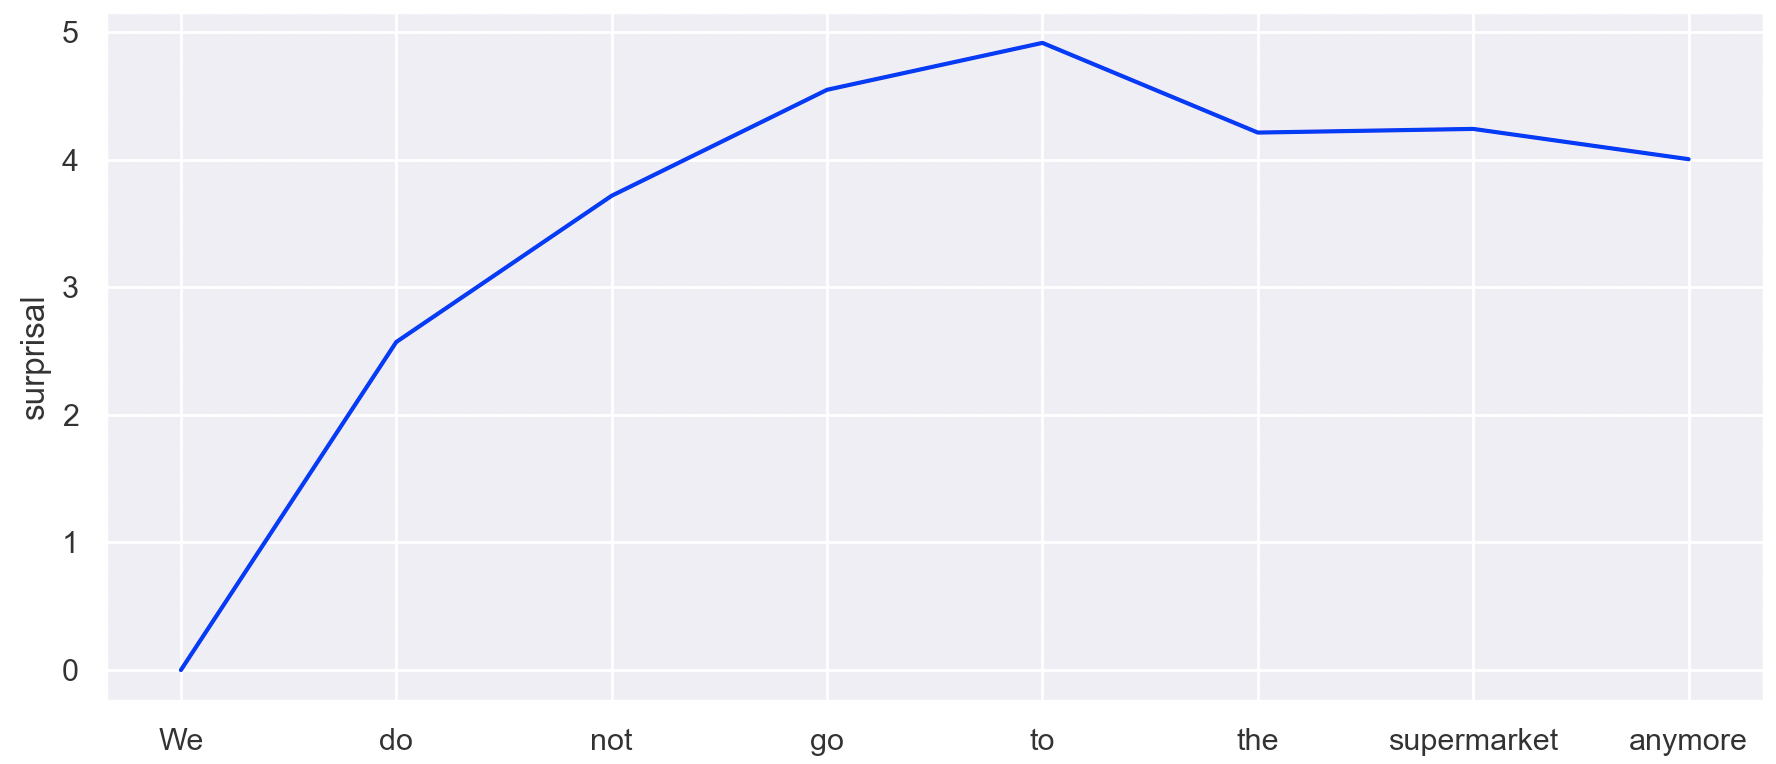
\includegraphics[width=.32\textwidth]{short} }}
    \subfloat[5 Additional Words]{{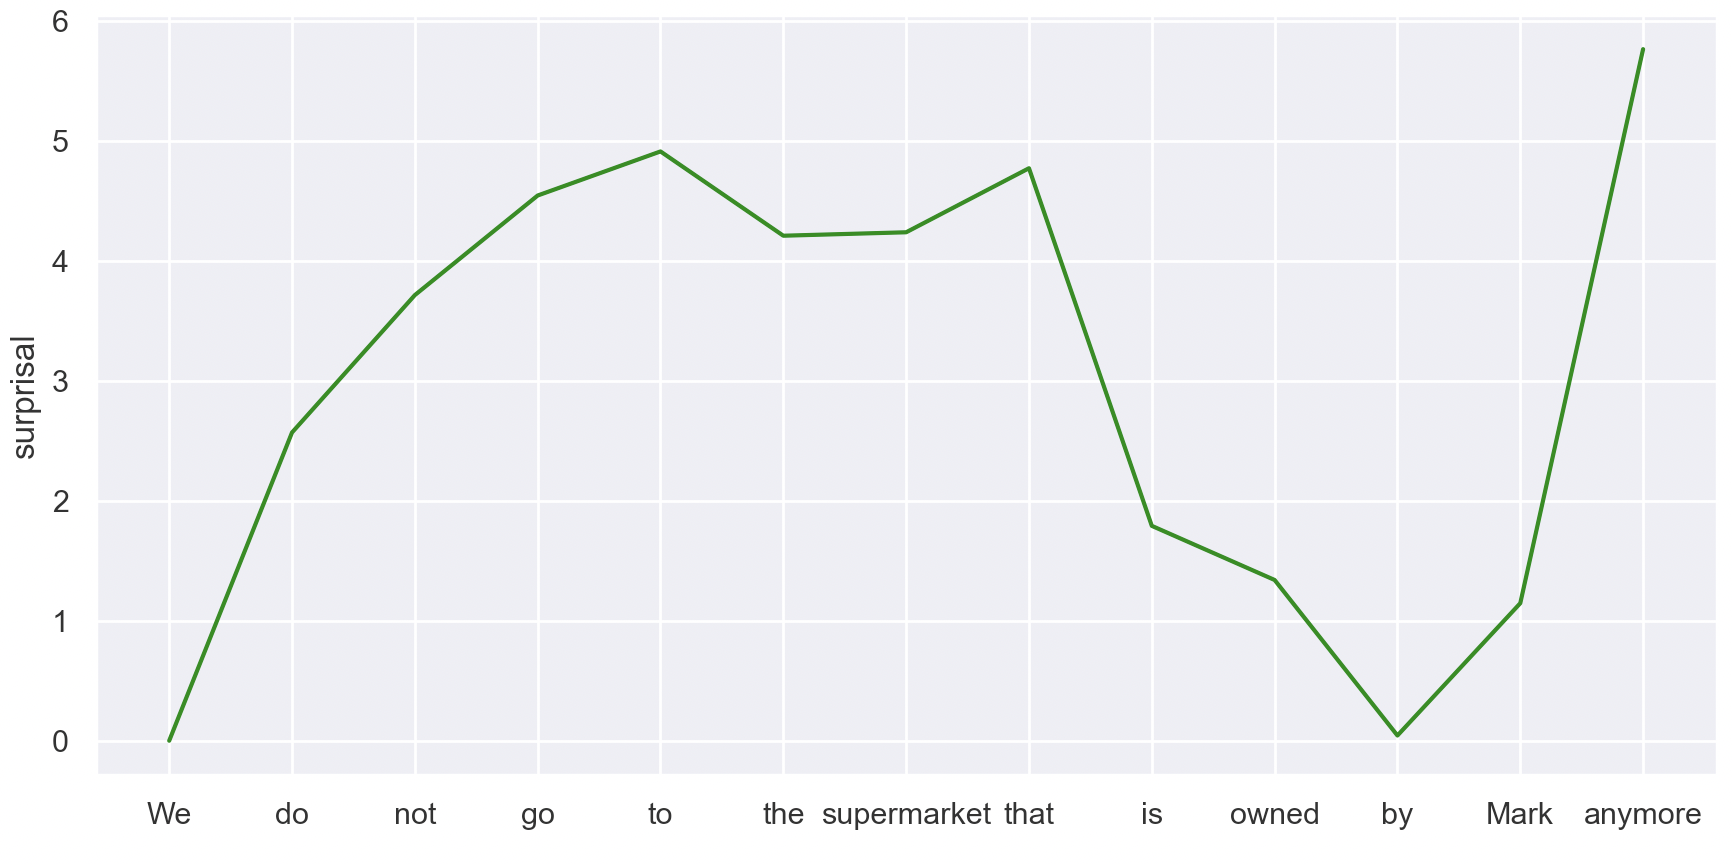
\includegraphics[width=.32\textwidth]{medium} }}
    \subfloat[8 Additional Words]{{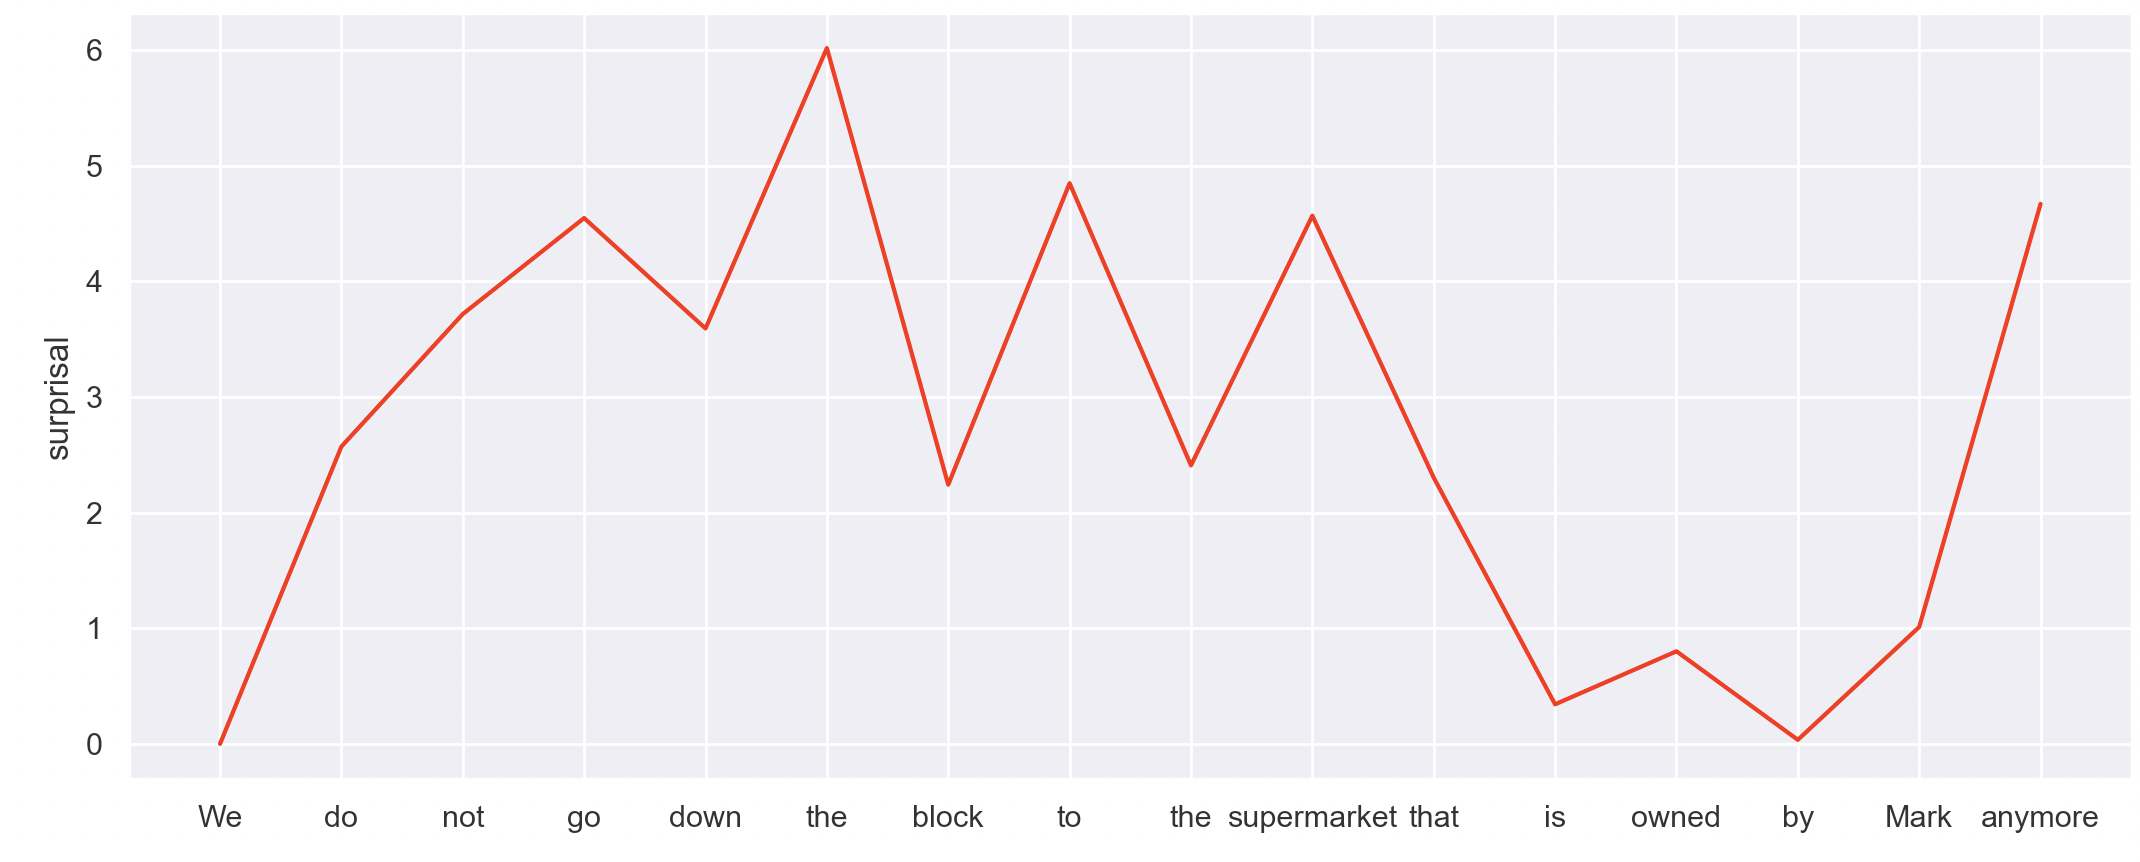
\includegraphics[width=.32\textwidth]{long} }}
    \caption{Plots of surprisal scores for words in the modified sentence. The surprisal score of the negative polarity item \textit{anymore} remains relatively unchanged by the amount of intervening material.}
    \label{fig:intervening2}
\end{figure*}
We also did a slightly different experiment aiming to control for variation in the semantic content of the sentences. Here, we designed 10 sentences base sentences with NPI items. Each of the base sentences comes in three varieties: minimal intervening material (enough to make the sentence grammatical), 3-5 words of additional intervening material, and 6-10 additional words between the negative licensor and the polarity item. In all cases the intervening words modify the object of the base sentence. An example of the results for this section are visualized in Figure \ref{fig:intervening2}.



We once again found that there was a weak positive correlation between amount of intervening material and the licensing interaction. However, as seen in the plots, the scores are relatively similar. This test supports the notation that the model's ability to predict the the distribution of NPIs is not affected by the quantity of intervening material.

% \subsection{Ability to License Multiple Negative Polarity Items}
% In most cases, a negative context can license multiple negative polarity items.
% \begin{exe}
% \ex
% \begin{xlist}
% \ex He didn't want to go with anybody anywhere
% \ex [*]{He did want to go with anybody anywhere} 
% \end{xlist}
% \end{exe} 
\section{Positive Polarity Items}
We briefly turn our attention to positive polarity items (PPIs) which are words that can only occur in ``positive'' contexts. English words such as \textit{some, rather,} and \textit{already} are common examples of PPIs. There is significantly less literature discussing PPIs than NPIs, and often the licensing of a positive context is much less explicit than that of a negative context. We are interested in whether LSTMs will exhibit higher surprisal in unlicensed settings, and if so, does the model understand PPIs to the same extent as NPIs. Establishing a positive context in English is not as explicit as establishing a negative context. Sentences default to the positive setting, and thus there is not an equivalent to \textit{not} which licenses a negative context. We hypothesize that the lack of an obvious licensor might make it more difficult for the model to determine whether a PPI is permissible.

\subsection{Licensing of Positive Polarity Items}
Positive polarity items may only be licensed in positive contexts, as is shown for the PPI \textit{rather} in the following example.
\begin{exe}
\ex \label{ex:positive}
\begin{xlist}
\ex I would rather be there
\ex[*]{I wouldn't rather be there} 


\end{xlist}
\end{exe}
Plotted in Figure \ref{fig:ppi-basic-licensing} are graphs surprisal of the sentences in \ref{ex:positive}. One can see that the positive polarity item has a slightly lower surprisal score in the grammatically correct context, but the trend is not as pronounced as what was seen with NPIs.

We conduct a nearly identical experiment as that in Section \ref{sec:basic} to determine the extent to which LSTMs learn about PPIs. We constructed 10 test items containing positive polarity items, and for each item, we constructed one with a positive context, and another with a negative context as exemplified in Example \ref{ex:positive}. If the model learned to predict PPIs only in positive contexts, then we would expect the licensing interaction of these sentences to be positive.

\begin{figure}
    \centering
    \subfloat[Grammatical]{{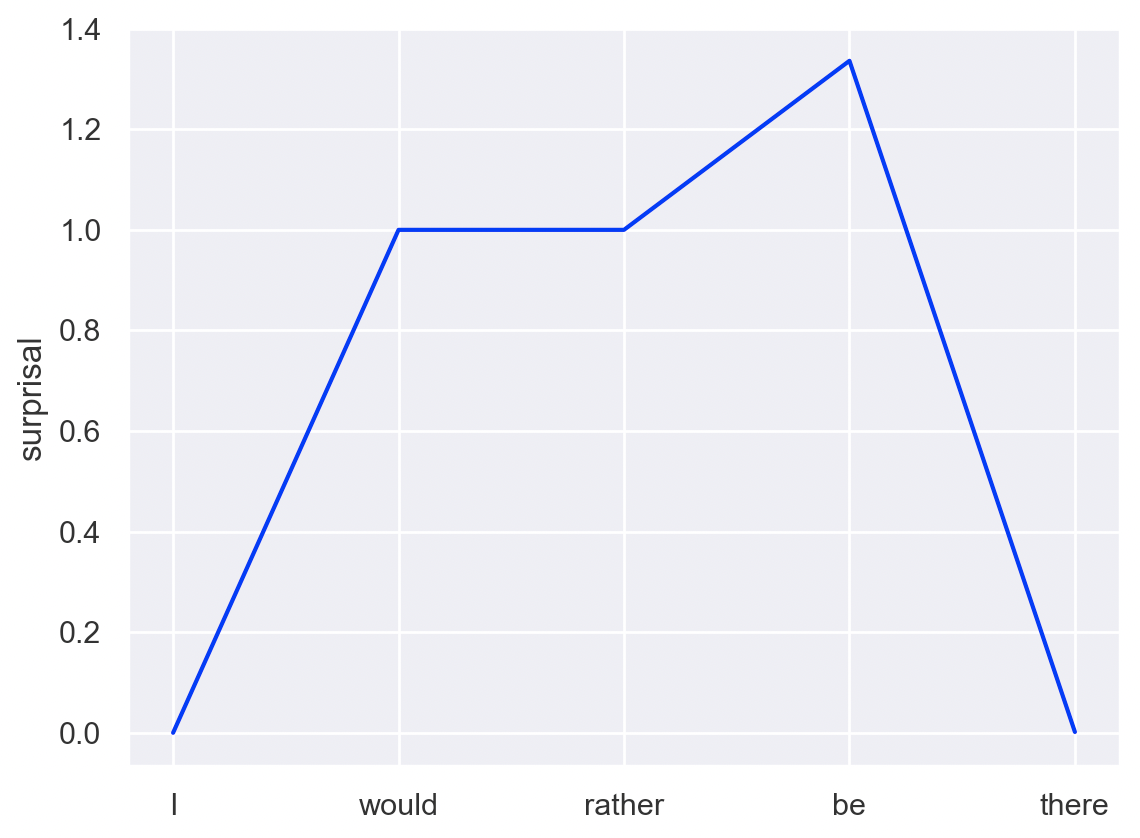
\includegraphics[width=.42\linewidth]{img/ppigood.png} }}
    \subfloat[Ungrammatical]{{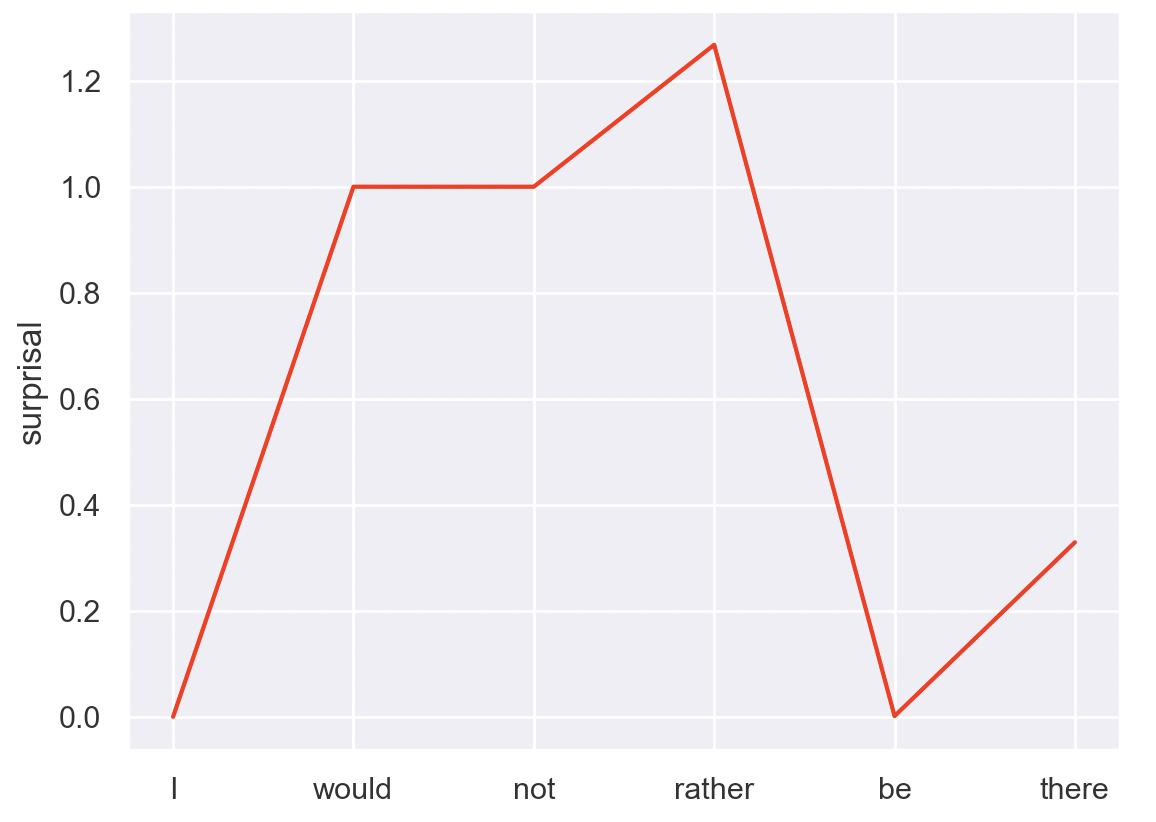
\includegraphics[width=.42\linewidth]{img/ppibad.png} }}
     \caption{The surprisal score for \textit{rather} is slightly lower in the positive context than in the incorrect negative context}
    \label{fig:ppi-basic-licensing}
\end{figure}

Measuring both instantaneous surprisal and cumulative surprisal after a PPI, we found in both cases that the mean licensing interaction is slightly greater than 0 (which implies that surprisal is higher when we find a PPI in a negative context), but the difference is not large enough to be statistically significant (instantaneous, $t(9) = 1.43$, $p = 0.093$; cumulative, $t(9) = 1.37$, $p = 0.102$). Thus, we fail to reject the null hypothesis that the licensing interaction is zero.

This small experiment suggests that it is more difficult for an LSTM to determine the validity of a PPI than an NPI. This result is not particularly surprising because, unlike NPIs, PPIs lack explicit licensors. Thus, in order to correctly predict the distribution of PPIs, the model would need to represent more complex aspects of language.

\section{Results and Discussion}

In Section \ref{sec:basic}, we showed that the presence of a negative licensor in a sentence caused a significant decrease in the model's surprisal upon encountering an NPI. This suggests that the model has learned that NPIs only occur when a negative licensor is present. However, in Section \ref{sec:c-command}, we saw that the model does not distinguish between licensors which c-command the NPI and those that do not. This suggests that, rather than representing the hierarchical structure of the sentence, the model approximates the NPI/licensor relation using a representation based on linear word order and precedence. Finally, in Section \ref{sec:intervening}, we saw that the model's ability to predict the distribution of NPIs was independent of the amount of intervening material.

Despite the fact that the experiments in Section \ref{sec:c-command} suggested that the model does not represent the c-command relation, the results do not differ too dramatically from what is observed in psycholinguistic studies of NPI licensing. As we would expect, listeners with no time constraints tend to judge sentences like those in Examples \ref{ex:c-command-np} and \ref{ex:c-command-pp} as being ungrammatical. However, when fast time constraints are placed on the judgement task, some speakers mistakenly accept sentences like Example \ref{ex:c-command-np} (in which there exists a negative licensor, but it is contained in an embedded clause) as grammatical \cite{xiang2009illusory,xiang2013dependency,parker2016negative}. This suggests that, under time pressure, the human brain might process the NPI licensing relation using a heuristic similar to the one that our model has learned, which takes into account only precedence and not c-command.

These results point towards a number of questions which could be addressed in future research. First of all, we might like to know how well these results generalize to other models. Our homegrown model was trained on a relatively small data set using limited resources; perhaps a larger LSTM like that presented in Jozefowicz et. al. \shortcite{jozefowicz2016exploring} would have a better chance of correctly modeling the c-command relationship. We could also apply a similar analysis to other types of network architectures, such as transformers. Large transformers like the GPT-2 model presented by Radford et. al. \shortcite{radford2019language} and the BERT model introduced in Devlin et. al. \shortcite{devlin2018bert} have both performed very well on a very general set of language modeling tasks. Repeating a similar analysis on GPT-2 or Bert could provide interesting insights into the extent to which transformer models represent hierarchical structure.

Of course, there is also further research that could be done without moving to a new model or architecture. One possibility would be to try to identify a specific unit or collection of units in the cell state of the LSTM that is responsible for tracking negative and positive states. This sort of analysis has been achieved before; in Lakretz et. al. \shortcite{lakretz2019emergence}, the authors identified discrete units responsible for tracking information about number agreement. They achieved this by using a technique known as \textit{ablation}. First, they constructed a task which measured the models ability to track number agreement. Then, one by one, they zeroed out (ablated) individual units in the LSTMs cell state. By selecting units whose ablation was associated with decreased success on the number agreement task, they were able to identify specific units responsible for tracking number agreement.

If a similar ablative analysis could identify specific units responsible for tracking negative polarity licensing, we could make predictions about how this unit's activation would change over the course of a sentence. In Section \ref{sec:c-command}, we observed that both embedded licensors and main licensors have a significant effect on surprisal, and that these effects combine linearly. This suggests that a hypothetical ``NPI licensing unit'' in the LSTM's hidden state should be expected to increase in activation each time the model encounters a negative word, regardless of the current level of activation. If we could observe this pattern in a specific unit of the LSTM's cell state, this would confirm that the unit identified by the ablative analysis was in fact responsible for tracking NPI licensing.

\section{Further Areas of Inquiry}

The processing of sentences producing Negative Polarity Illusions remains a remarkably interesting open area of inquiry. Such illusions refer to sentences wherein there is an illusory licensing of agreement and negative polarity items, in that sentences with unlicensed agreement or an unlicensed NPI are perceived as comprehensible and acceptable upon first utterance but upon further reflection are judged as unacceptable due to faulty licensing. Analyzing if LSTM models are able to distinguish in instinctive licensing "correctness," wherein sentences non-illusory sentences are perceived as acceptable or unacceptable strictly contingent upon licensing and illusory sentences are perceived as acceptable or unacceptable in a more loosely fashion, is a goal for further research.

\bibliography{sources}

\end{document}
